\chapter{Release 1}
\label{chap:release1}

\section{Introduction}
\label{sec:release1-intro}

Release 1 presents the first three sprints of the Production Tracker project, focusing on building a solid foundation with authentication and access control, implementing the core production flow, and developing an inventory management system. This release provides the essential features needed to track work orders and manage stock efficiently.

\section{Sprint 1: Foundation and Access Control}
\label{sec:sprint1}

\subsection{Sprint 1 Backlog}
\label{sec:sprint1-backlog}
the table \ref{tab:sprint1-backlog} summarizes the user stories and tasks completed during Sprint 1.
\footnotesize
\begin{longtable}{|p{0.10\textwidth}|p{0.50\textwidth}|p{0.32\textwidth}|}
    \caption{Sprint 1 Backlog}\label{tab:sprint1-backlog}\\
    \hline
    \textbf{ID} & \textbf{User Story} & \textbf{Tasks} \\
    \hline
    \endfirsthead
    \hline
    \textbf{ID} & \textbf{User Story} & \textbf{Tasks} \\
    \hline
    \endhead
    \hline
    \endfoot
    PB-01 & As an administrator, I want to log in securely so that I can access protected features. & Setup authentication module; \newline   Implement login/logout; \newline Add password hashing \\
    \hline
    PB-02 & As an administrator, I want role-based permissions so that users access only appropriate features. & Define role models; \newline  Implement permission checks; \newline  Create role management UI \\
    \hline
    PB-03 & As an administrator, I want to create and manage user accounts so that the team can access the system. & Build user CRUD operations; \newline  Add user validation; \newline  Create user management interface \\
    \hline
    PB-04 & As a user, I want secure session handling so that my account remains protected. & Implement JWT tokens; \newline  Add session expiration; \newline  Create token refresh mechanism \\
    \hline
\end{longtable}
\normalsize
\subsection{Sprint 1 use case diagram}
the figure \ref{fig:sprint1-use-case-diagram} illustrates the main use cases implemented in Sprint 1, focusing on user authentication and management features. It shows the interactions between the administrator and the system for logging in, and managing user accounts.
\begin{figure}[H]
    \centering
    
    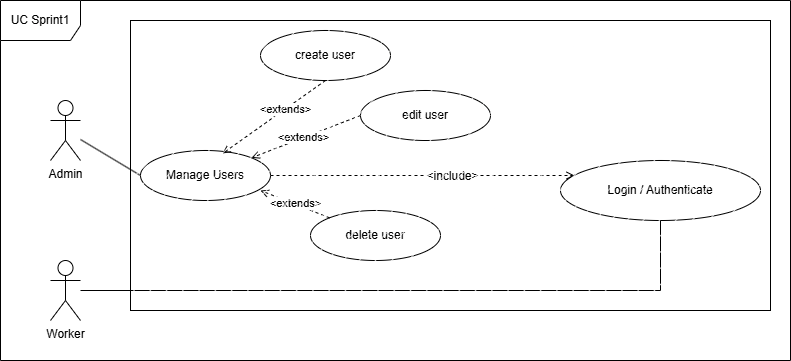
\includegraphics[width=\textwidth,keepaspectratio]{pictures/sprint1 use case diagarm.drawio.png}
    \vspace*{\fill}
    \caption{Sprint 1 Use Case Diagram}
    \label{fig:sprint1-use-case-diagram}
\end{figure}
\subsection{User Login and Protected Resource Access — JWT Sequence Diagram}
    JSON Web Token (JWT) is a proposed Internet standard for creating data with optional signature and/or optional encryption whose payload holds JSON that asserts some number of claims. The tokens are signed either using a private secret or a public/private key. \hyperref[ref:jwt]{[20]} 

the figure \ref{fig:jwt-sequence-diagram} illustrates the sequence of interactions during the authentication process using JWT tokens. 

\begin{figure}[H]
    \centering
    
    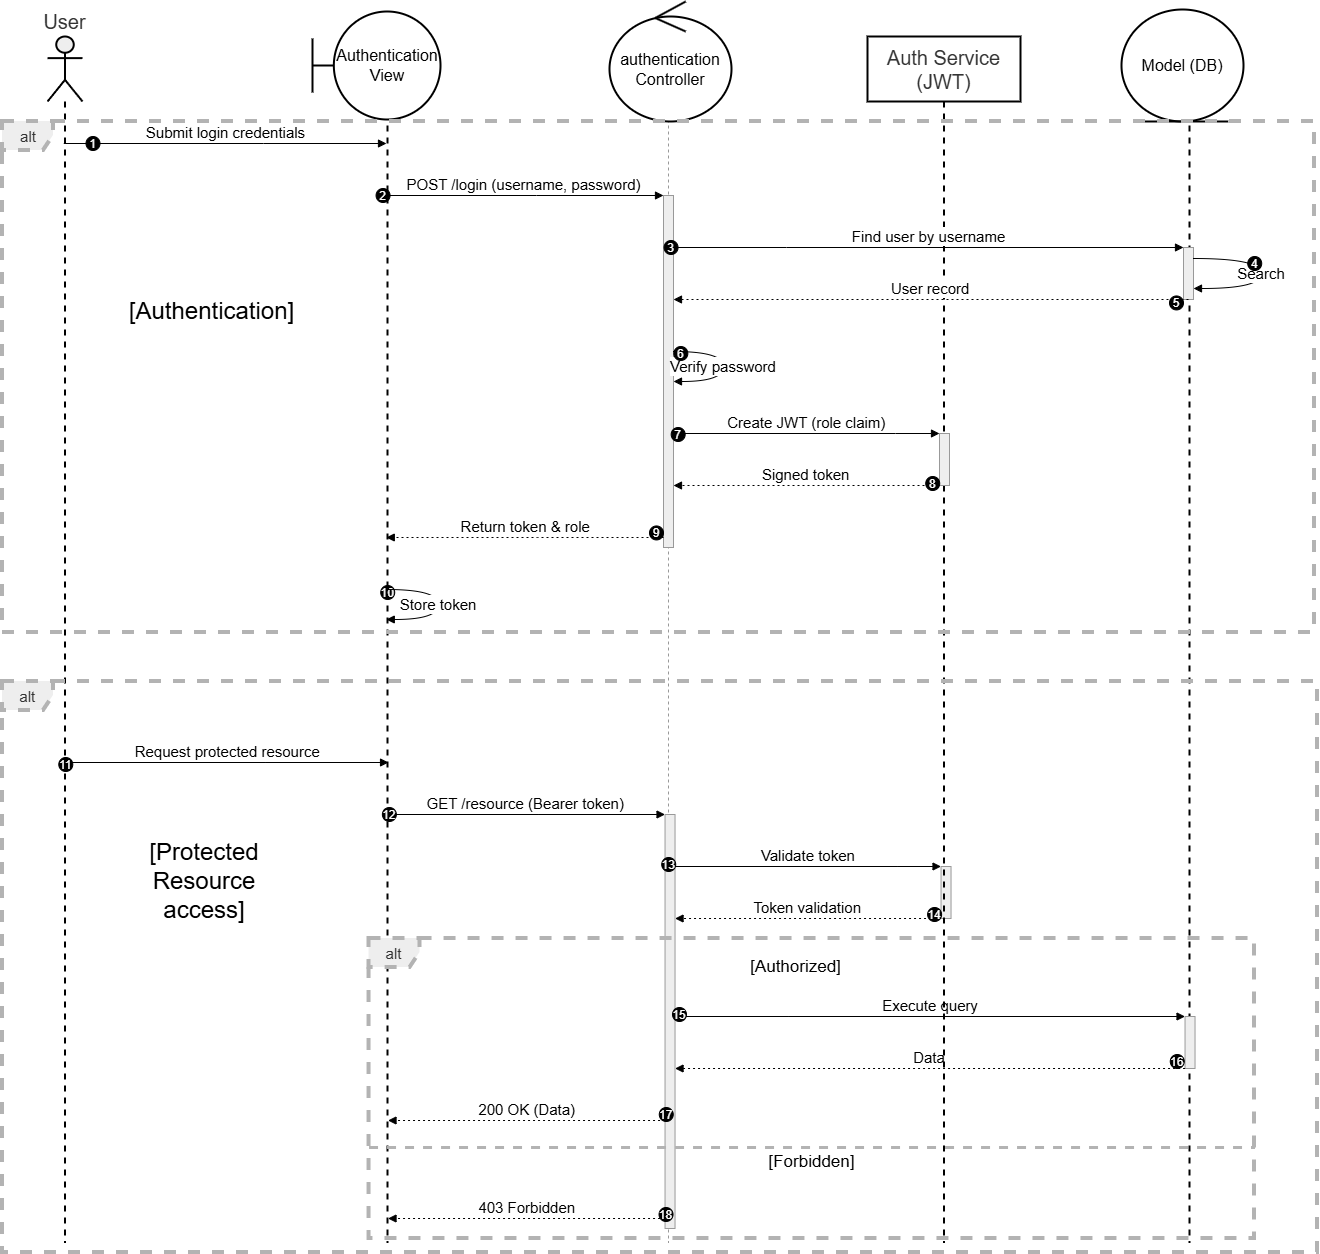
\includegraphics[width=\textwidth,keepaspectratio]{pictures/jwt authentication sequence diagram.drawio.png}
    \vspace*{\fill}
    \caption{Authentication Sequence Diagram}\label{fig:jwt-sequence-diagram}
\end{figure}


\subsection{Sprint 1: Application Interface Overview}
\label{sec:sprint1-interfaces}
The figure \ref{fig:login-interface} show the login interface that represents the gate to access the platform.
While the figures \ref{fig:user-management-interface} and \ref{fig:user-creation-modal} show the user management interface that allows administrators to create and manage user accounts, including a modal for creating new users with role assignments and validation features.
\begin{figure}[H]
    \centering
    
    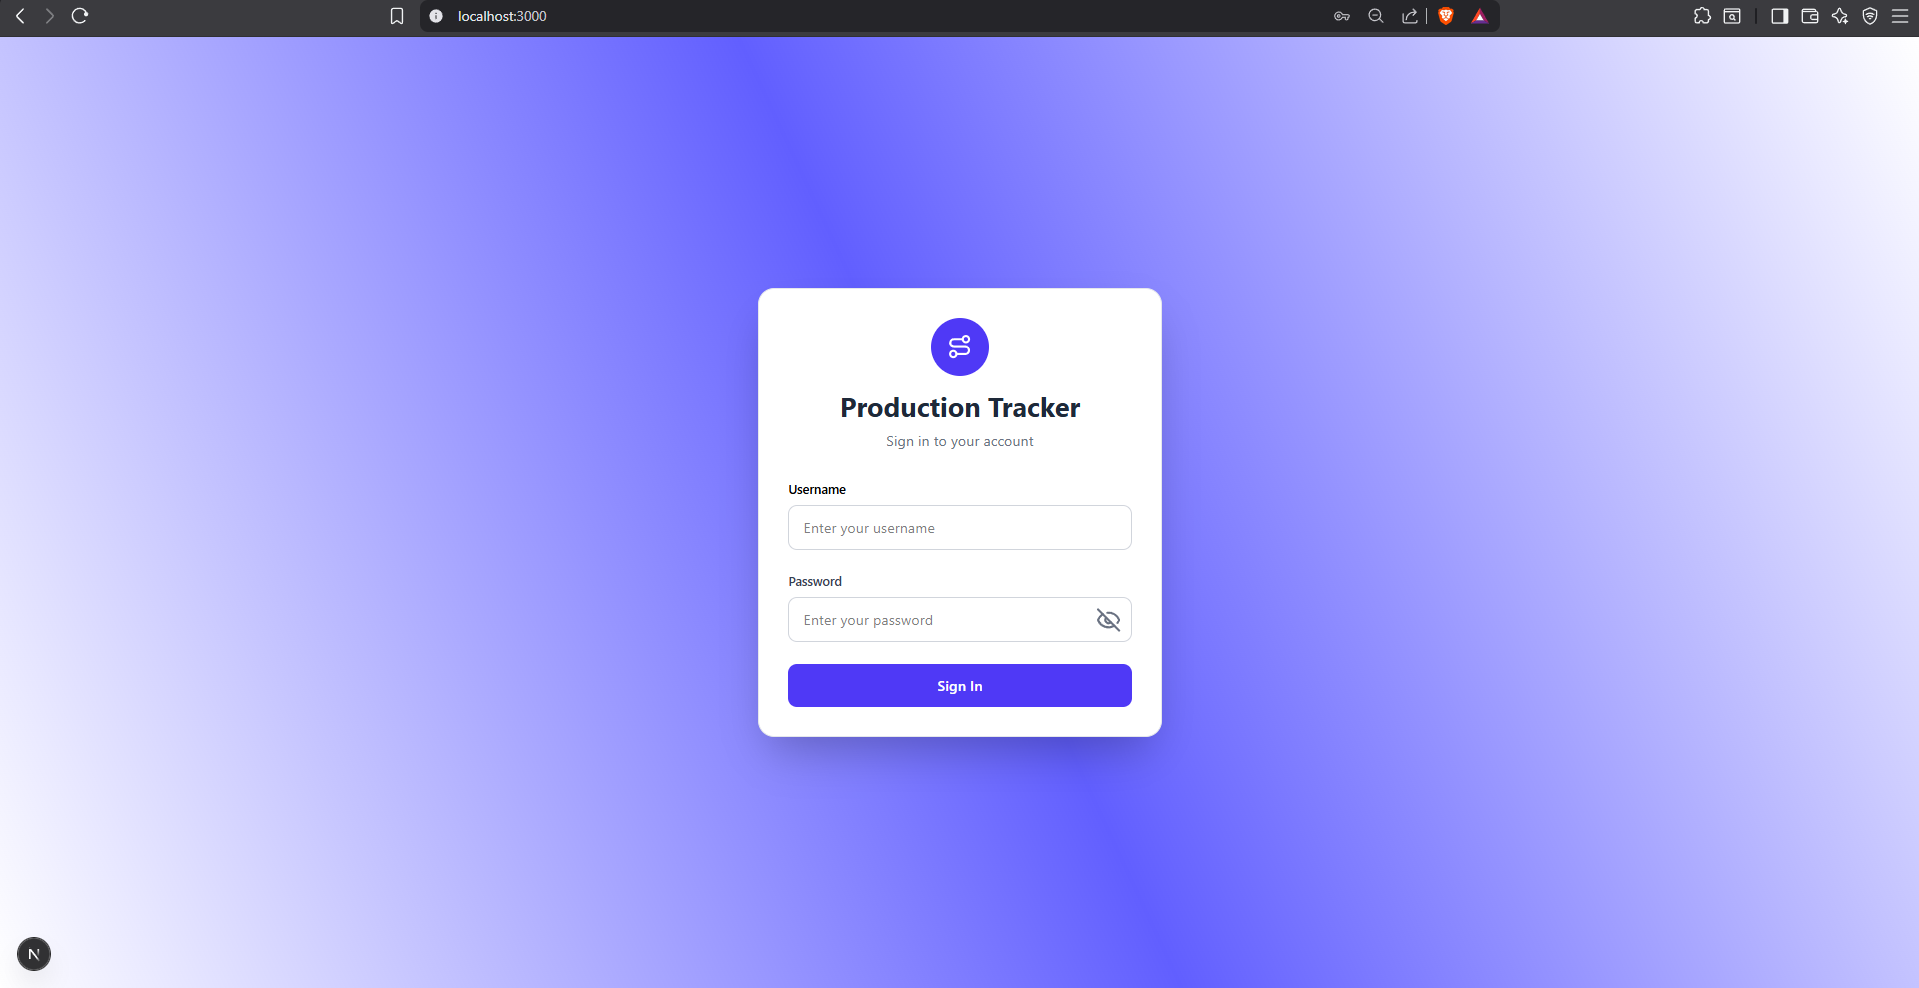
\includegraphics[width=\textwidth,keepaspectratio]{pictures/login-interface.png}
    \vspace*{\fill}
    \caption{Login Interface} \label{fig:login-interface}
\end{figure}
\begin{figure}[H]
    \centering

    \begin{minipage}[t]{0.48\textwidth}
        \centering
        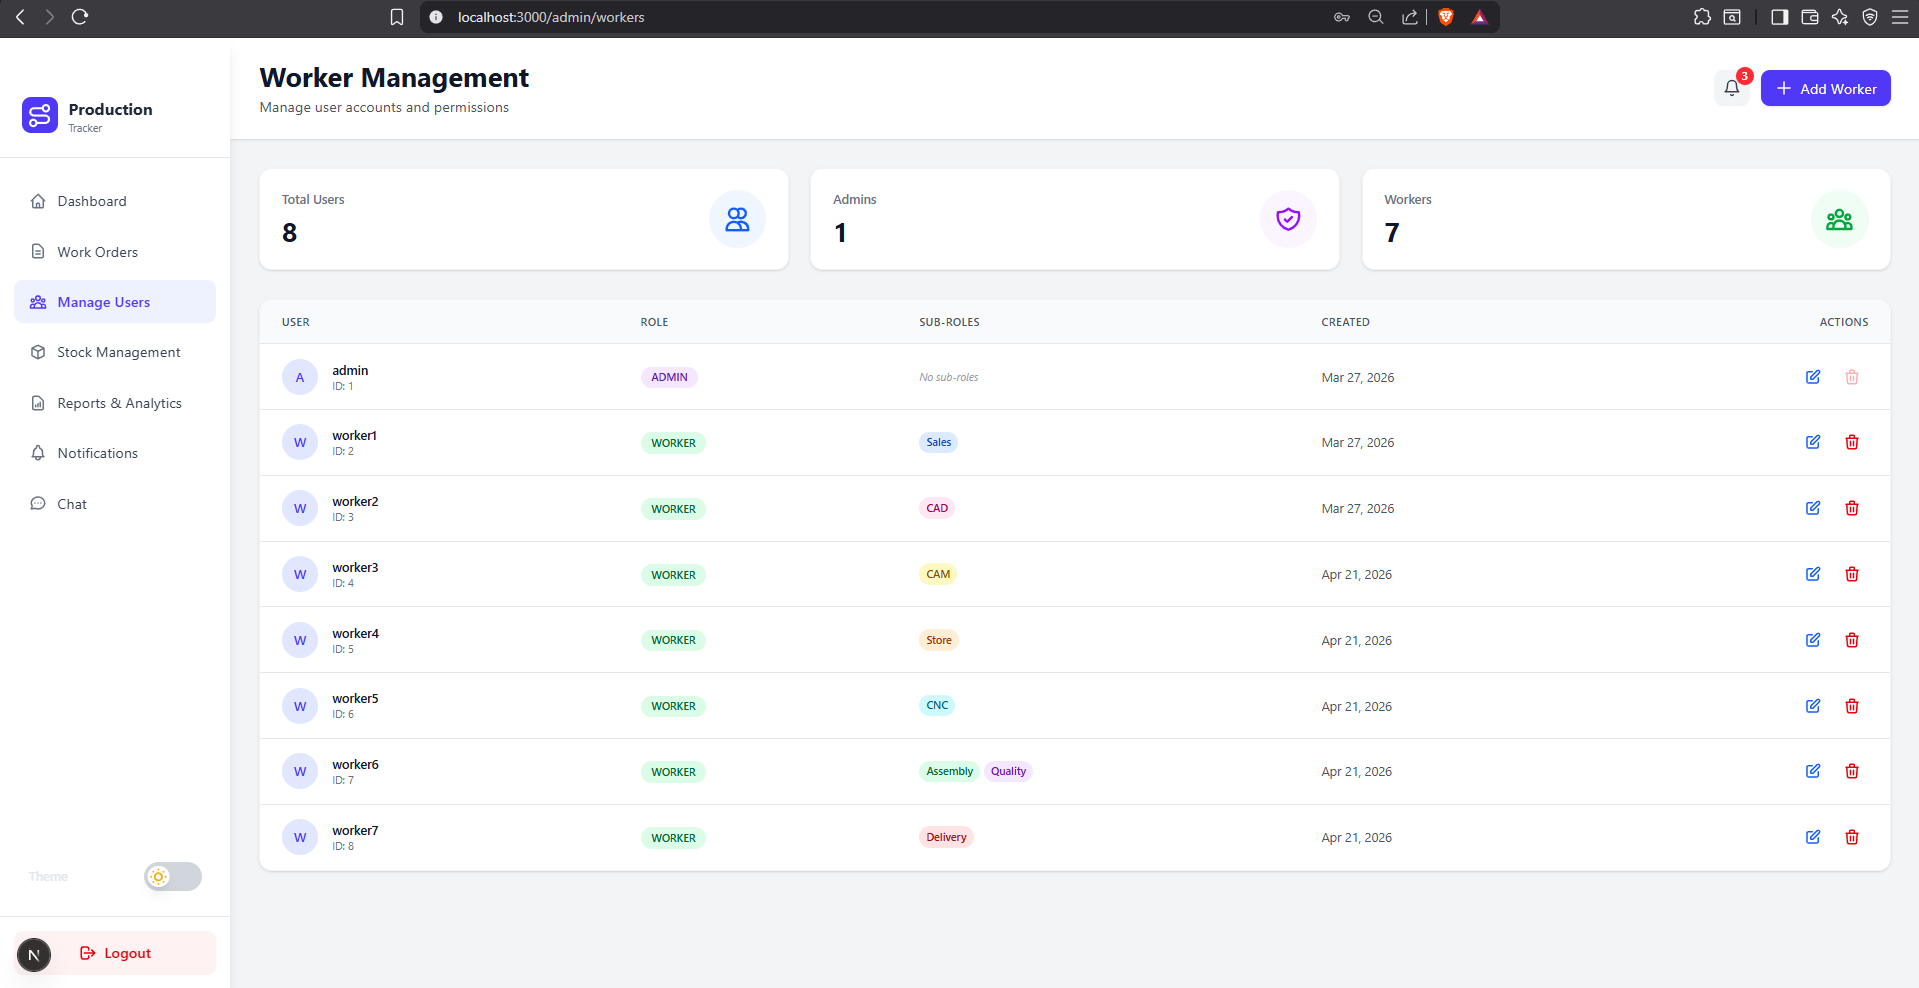
\includegraphics[width=\textwidth]{pictures/user managment interface.png}
        \caption{User Management Interface}
        \label{fig:user-management-interface}
    \end{minipage}
    \hfill
    \begin{minipage}[t]{0.48\textwidth}
        \centering
        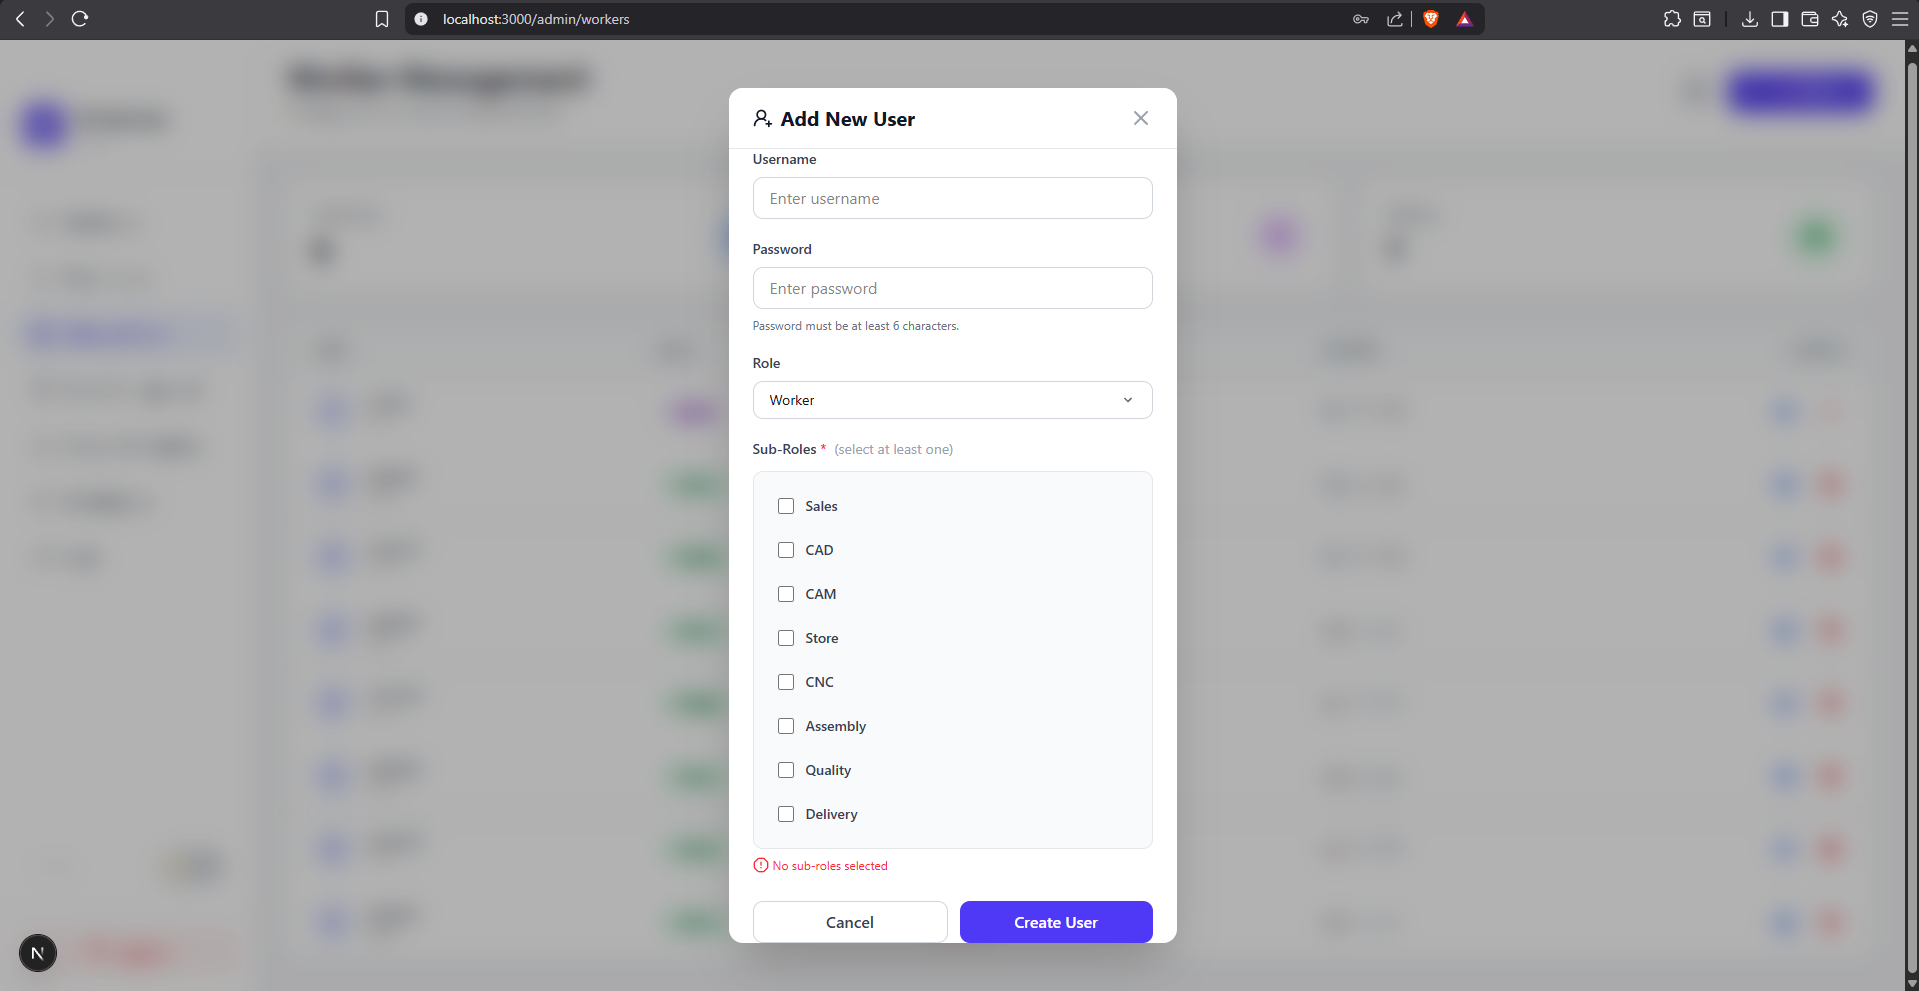
\includegraphics[width=\textwidth]{pictures/user creation modal.png}
        \caption{User Creation Modal}
        \label{fig:user-creation-modal}
    \end{minipage}

\end{figure}

\section{Sprint 2: Work Orders and Stage Tracking}
\label{sec:sprint2}

\subsection{Sprint Backlog}
\label{sec:sprint2-backlog}


the table \ref{tab:sprint2-backlog} summarizes the user stories and tasks completed during Sprint 2.
\begin{longtable}{|p{0.10\textwidth}|p{0.50\textwidth}|p{0.32\textwidth}|}
    \caption{Sprint 2 Backlog}\label{tab:sprint2-backlog}\\
    \hline
    \textbf{ID} & \textbf{User Story} & \textbf{Tasks} \\
    \hline
    \endfirsthead
    \hline
    \textbf{ID} & \textbf{User Story} & \textbf{Tasks} \\
    \hline
    \endhead
    \hline
    
    \endfoot
    
    PB-05 & As an administrator, I want to create work orders with all required details so that tasks are clearly defined. & Design work order schema; \newline  Build creation form; \newline  Add validation and error handling \\
    \hline
    PB-06 & As an administrator, I want to assign work orders to workers so that each task has a responsible person. & Create assignment workflow; \newline  Build assignment UI; \newline  Add notification trigger \\
    \hline
    PB-07 & As a worker, I want to update my work order status so that progress is visible in real time. & Build status update endpoints; \newline  Create status UI; \newline Add real-time updates \\
    \hline
\end{longtable}
\normalsize
\subsection{ Sprint 2 use case diagram}
the figure \ref{fig:sprint2-use-case-diagram} illustrates the main use cases implemented in Sprint 2, focusing on work order management and stage tracking features. It shows the interactions between the administrator and workers with the system for creating, assigning, and updating work orders.
\begin{figure}[H]
    \centering
    
    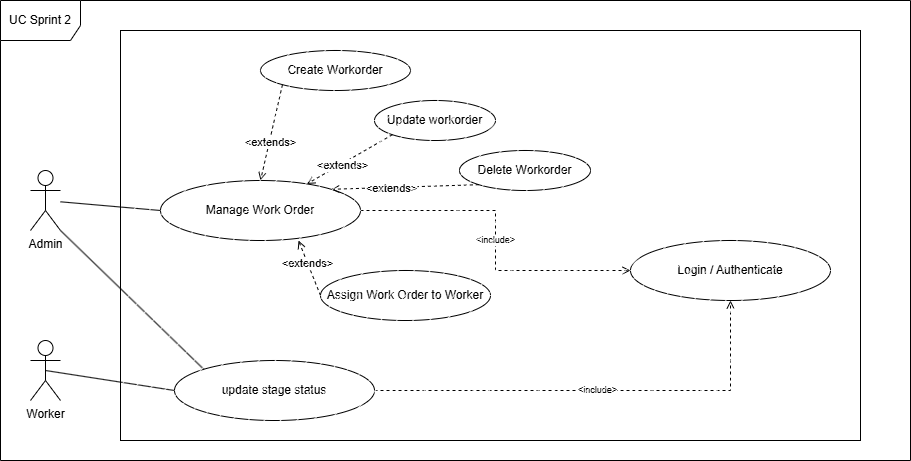
\includegraphics[width=\textwidth,keepaspectratio]{pictures/Sprint2 use case diagram.drawio.png}
    \vspace*{\fill}
    \caption{Sprint 2 Use Case Diagram}
    \label{fig:sprint2-use-case-diagram}
\end{figure}

\subsection{ Sequence Diagram for Work Order Progress Update}
the figure \ref{fig:work-order-sequence-diagram} illustrates the sequence of interactions during the work order progress update process, showing how a worker updates the status of a work order and how the system processes this update to reflect changes in the production workflow.
\begin{sidewaysfigure}
    \centering
    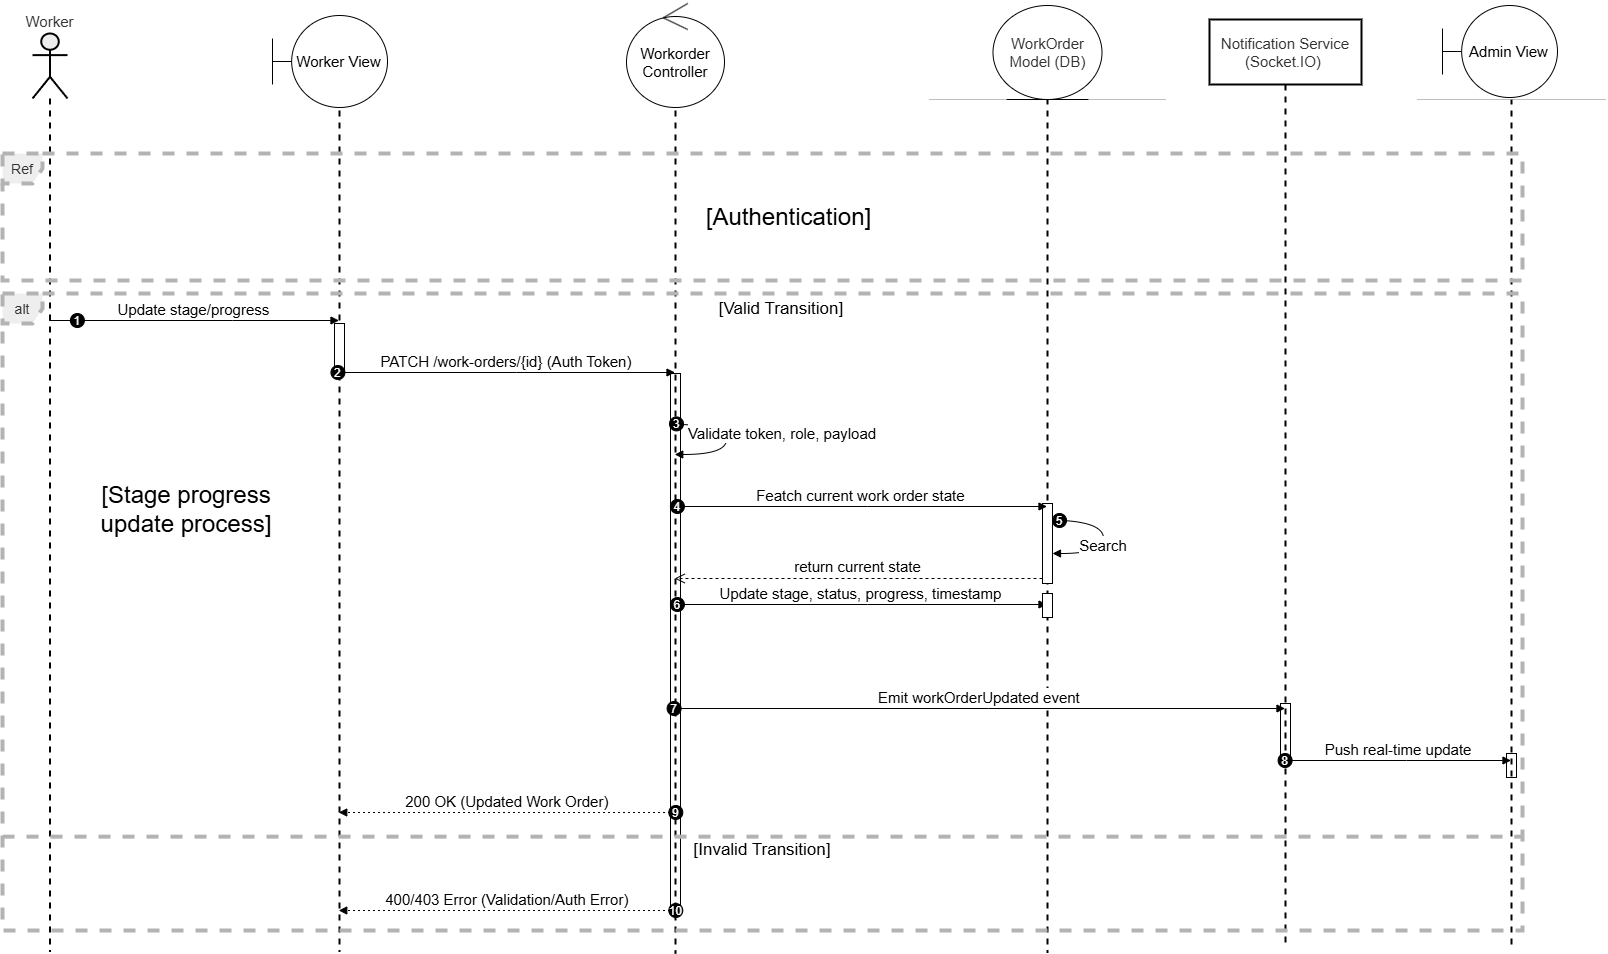
\includegraphics[width=0.95\textheight]{pictures/Work order stage_progress update.drawio.png}
    \caption{Work Order Progress Update Sequence Diagram}
    \label{fig:work-order-sequence-diagram}
\end{sidewaysfigure}

\subsection{Sprint 2: Application Interface Overview}
\label{sec:sprint2-interfaces}

the figures \ref{fig:work-order-management-interface}, \ref{fig:production-stages-admin}, and \ref{fig:worker-tasks-view} show the interfaces related to work order management, production stages administration, and worker task views, respectively. These interfaces allow administrators to manage work orders and production stages while providing workers with a clear view of their assigned tasks and progress.
\begin{figure}[H]
    \centering
    
    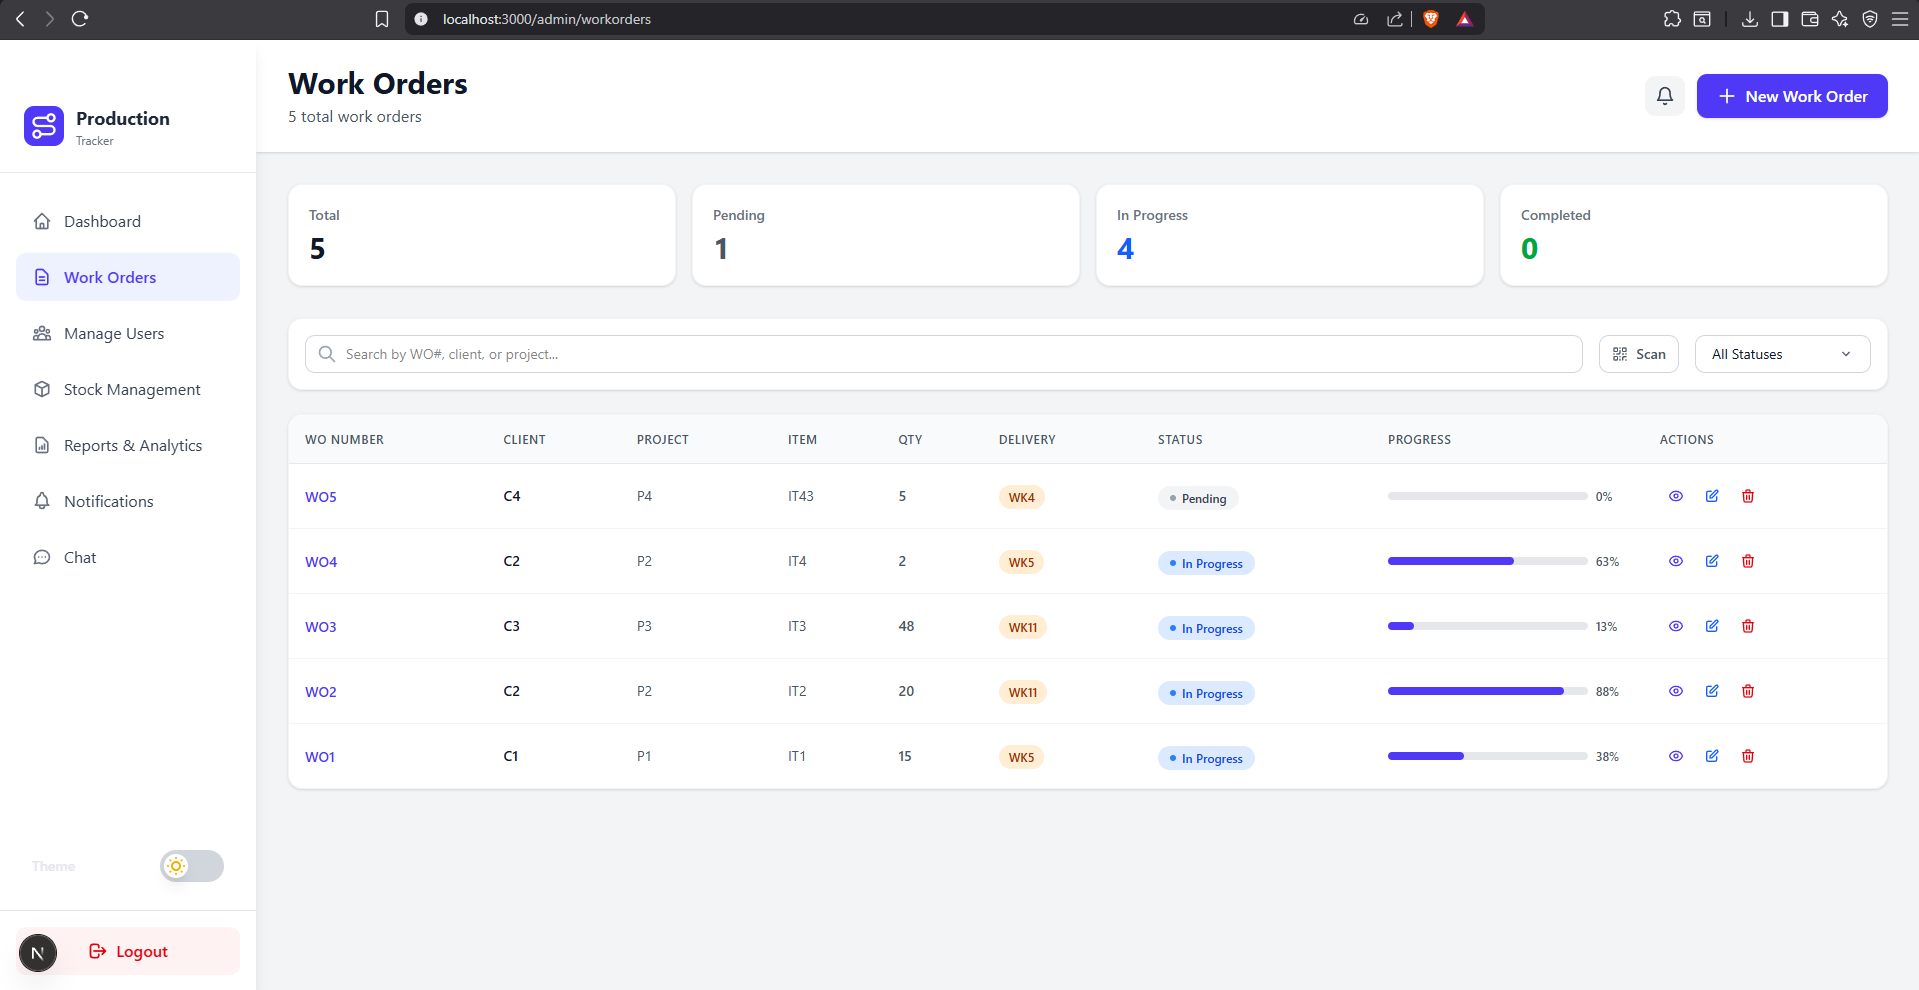
\includegraphics[width=\textwidth,keepaspectratio]{pictures/Workorder managment interface.png}
    \vspace*{\fill}
    \caption{Work Order Management Interface}
    \label{fig:work-order-management-interface}
\end{figure}
\begin{figure}[H]
    \centering

    \begin{minipage}[t]{0.48\textwidth}
        \centering
        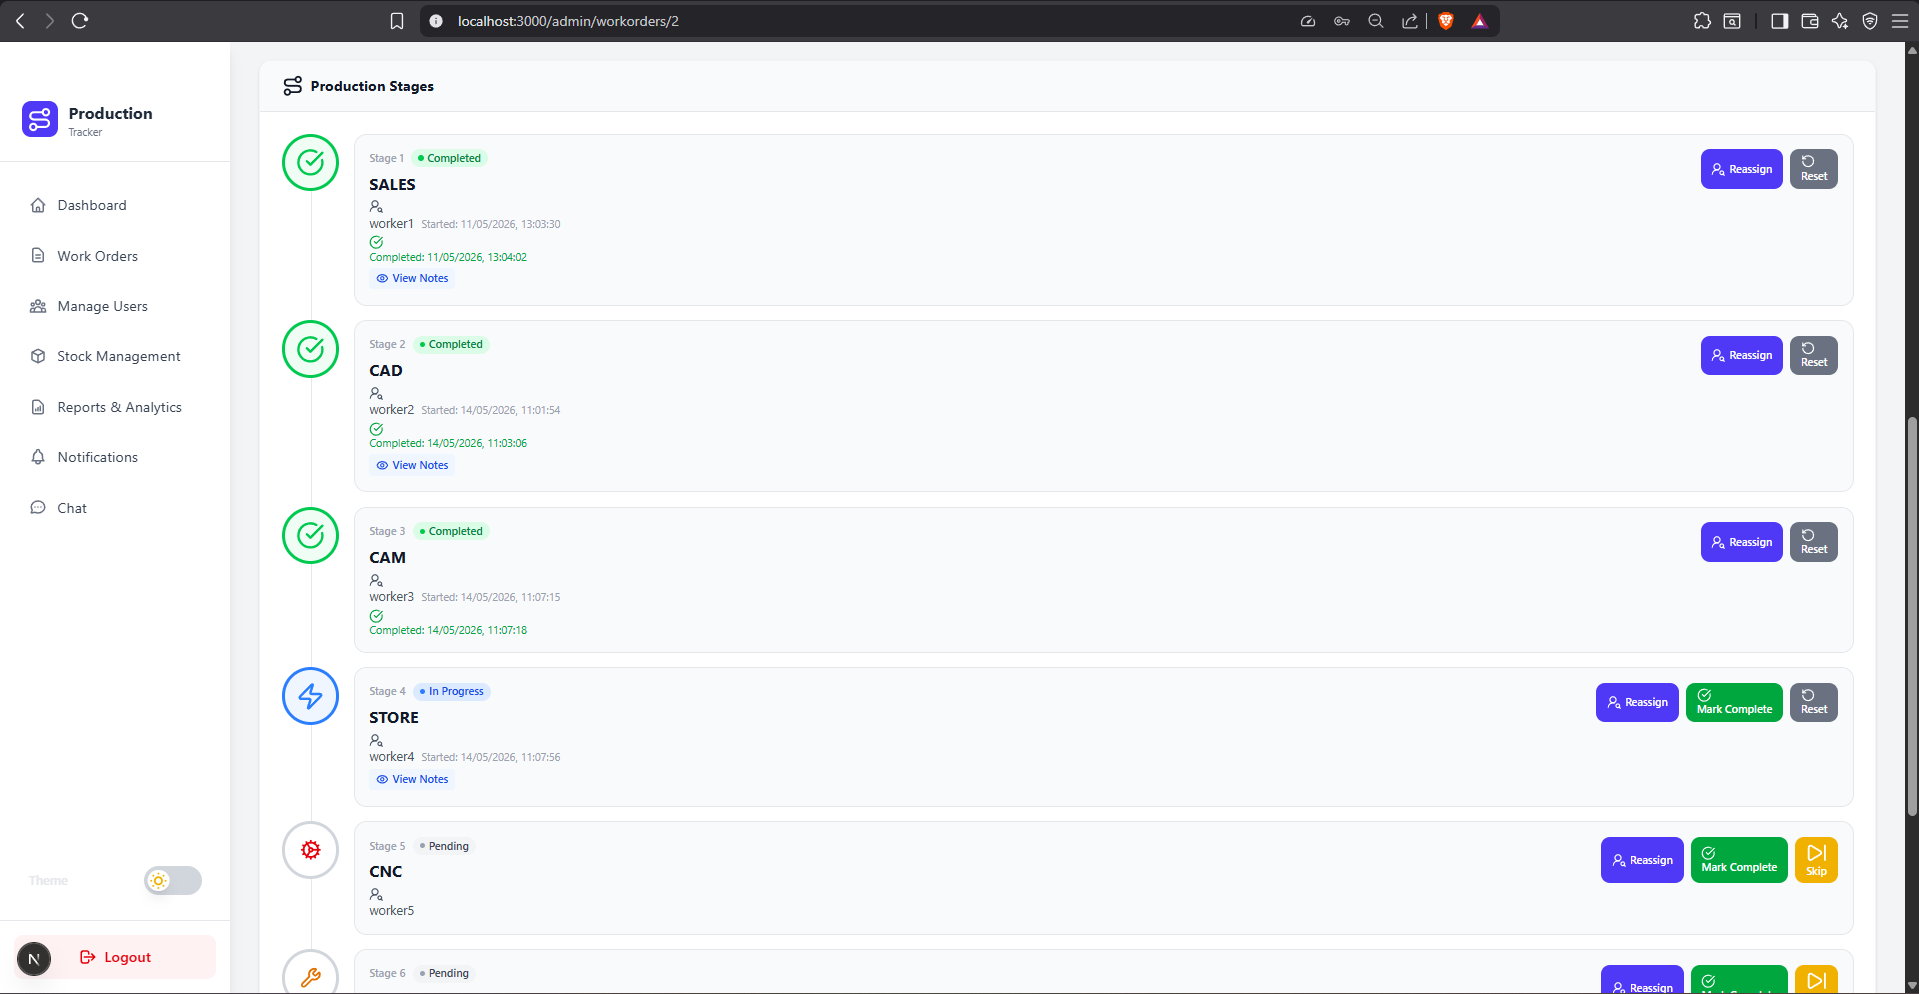
\includegraphics[width=\textwidth,keepaspectratio]{pictures/production stages admin view.png}
        \caption{Production Stages Admin View}
        \label{fig:production-stages-admin}
    \end{minipage}
    \hfill
    \begin{minipage}[t]{0.48\textwidth} 
        \centering
        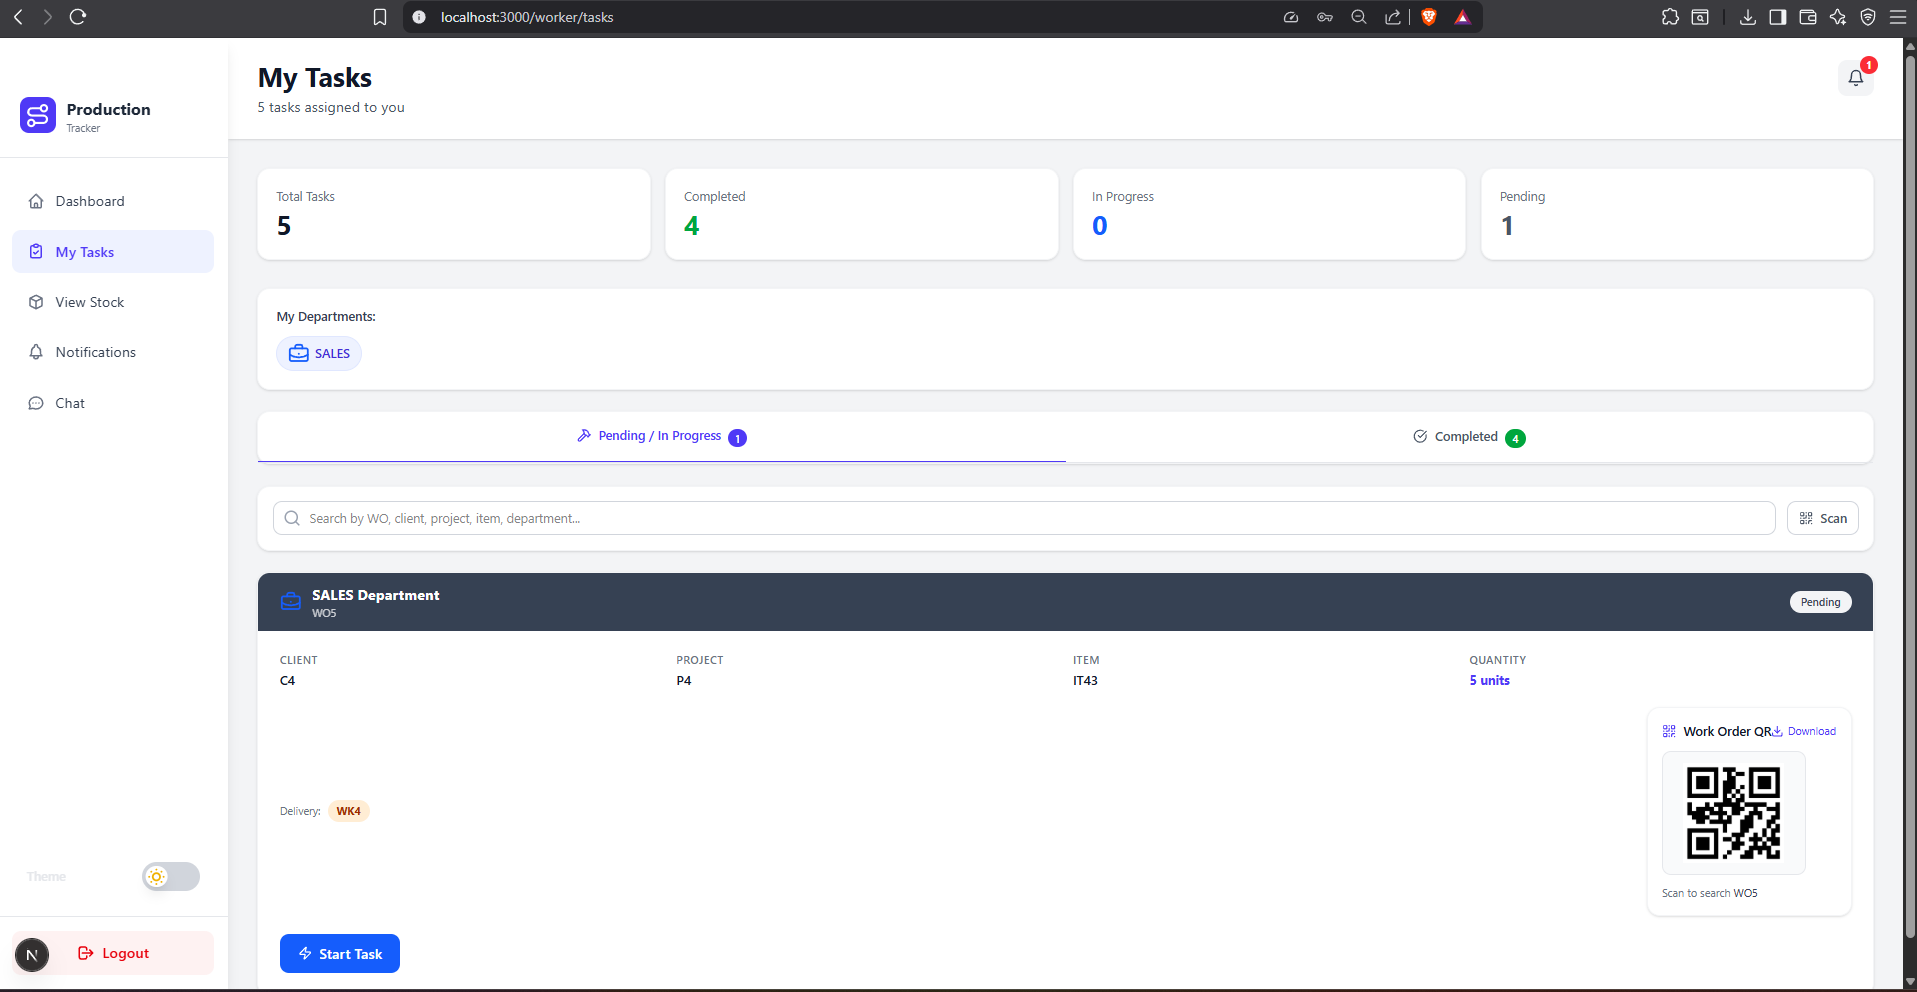
\includegraphics[width=\textwidth,keepaspectratio]{pictures/worker tasks view.png}
        \caption{Worker Tasks View}
        \label{fig:worker-tasks-view}
    \end{minipage}

\end{figure}
\section{Sprint 3: Stock Management}
\label{sec:sprint3}

\subsection{Sprint Backlog}
\label{sec:sprint3-backlog}
the table \ref{tab:sprint3-backlog} summarizes the user stories and tasks completed during Sprint 3.
\footnotesize
\begin{longtable}{|p{0.10\textwidth}|p{0.50\textwidth}|p{0.32\textwidth}|}
    \hline
    \textbf{ID} & \textbf{User Story} & \textbf{Tasks} \\
    \hline
    \endfirsthead
    \hline
    \textbf{ID} & \textbf{User Story} & \textbf{Tasks} \\
    \hline
    \endhead
    \hline
    \endfoot
    PB-08 & As an admin, I want to create, edit, and delete stock items so that inventory stays accurate. & Design inventory schema; \newline  Build stock registration UI; \newline  create Stock CRUD works \\
    \hline
    PB-09 & As a worker, I want to reserve stock items for my tasks and mark them as consumed when used. & create reservation logic; \newline  build reservation interface;  \\
    \hline
    PB-10 & As an administrator, I want to monitor stock reservations &  create reservation tracking functionality; \newline Build reservation tracking UI;\\
    \hline
    \caption{Sprint 3 Backlog}\label{tab:sprint3-backlog}\\
\end{longtable}
\normalsize

\subsection{Sprint 3 use case diagram}
the figure \ref{fig:sprint3-use-case-diagram} illustrates the main use cases implemented in Sprint 3, focusing on stock management features. It shows the interactions between administrators and workers with the system for managing stock items, reserving inventory, and monitoring reservations.
\begin{figure}[H]
    \centering
    
    \includegraphics[width=\textwidth,keepaspectratio]{pictures/sprint3 use case diagram.drawio.png}
    \vspace*{\fill}
    \caption{Sprint 3 Use Case Diagram}
    \label{fig:sprint3-use-case-diagram}
\end{figure}


\subsection{Sprint 3: Application Interface Overview}
\label{sec:sprint3-interfaces}
the figures \ref{fig:inventory-admin-view} and \ref{fig:inventory-reservations-admin-view} show the inventory management interfaces for administrators, allowing them to manage stock items and monitor reservations. 
\begin{figure}[H]
    \centering

    \begin{minipage}[t]{0.48\textwidth}
        \centering
        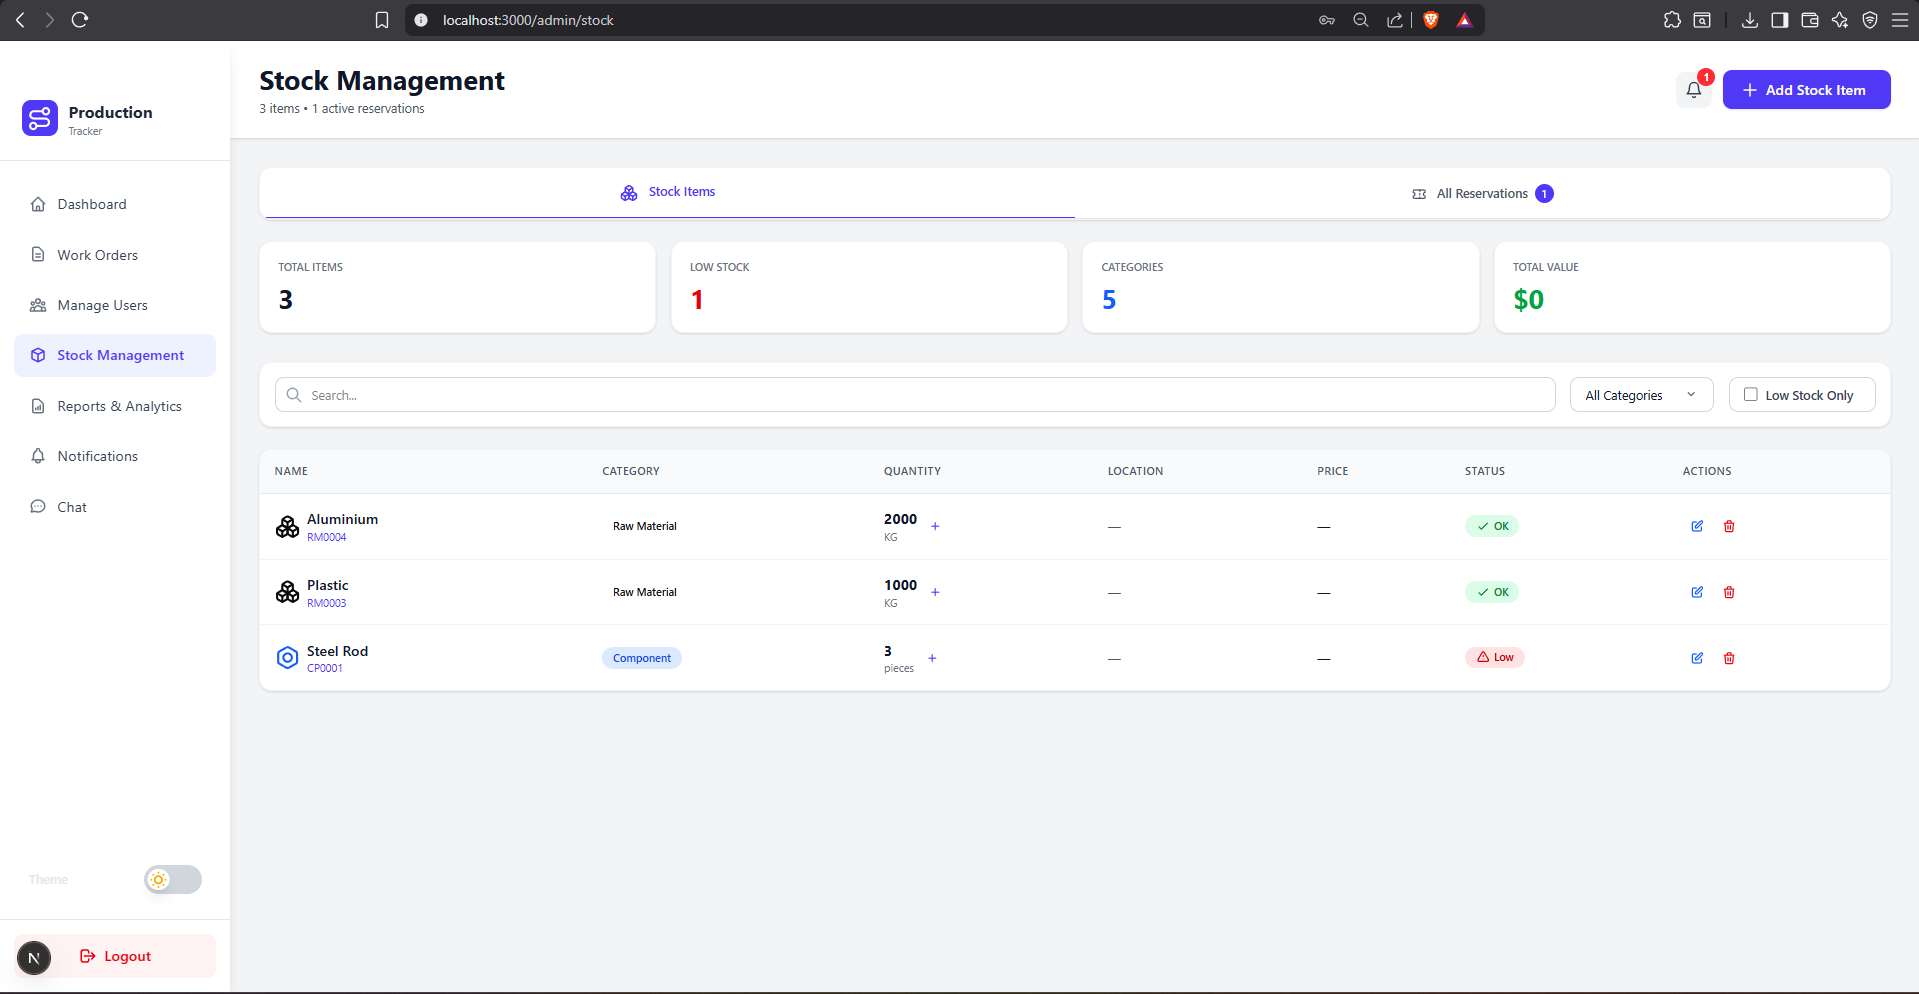
\includegraphics[width=\textwidth,keepaspectratio]{pictures/inventory admin view.png}
        \caption{Inventory Admin View}
        \label{fig:inventory-admin-view}
    \end{minipage}
    \hfill
    \begin{minipage}[t]{0.48\textwidth} 
        \centering
        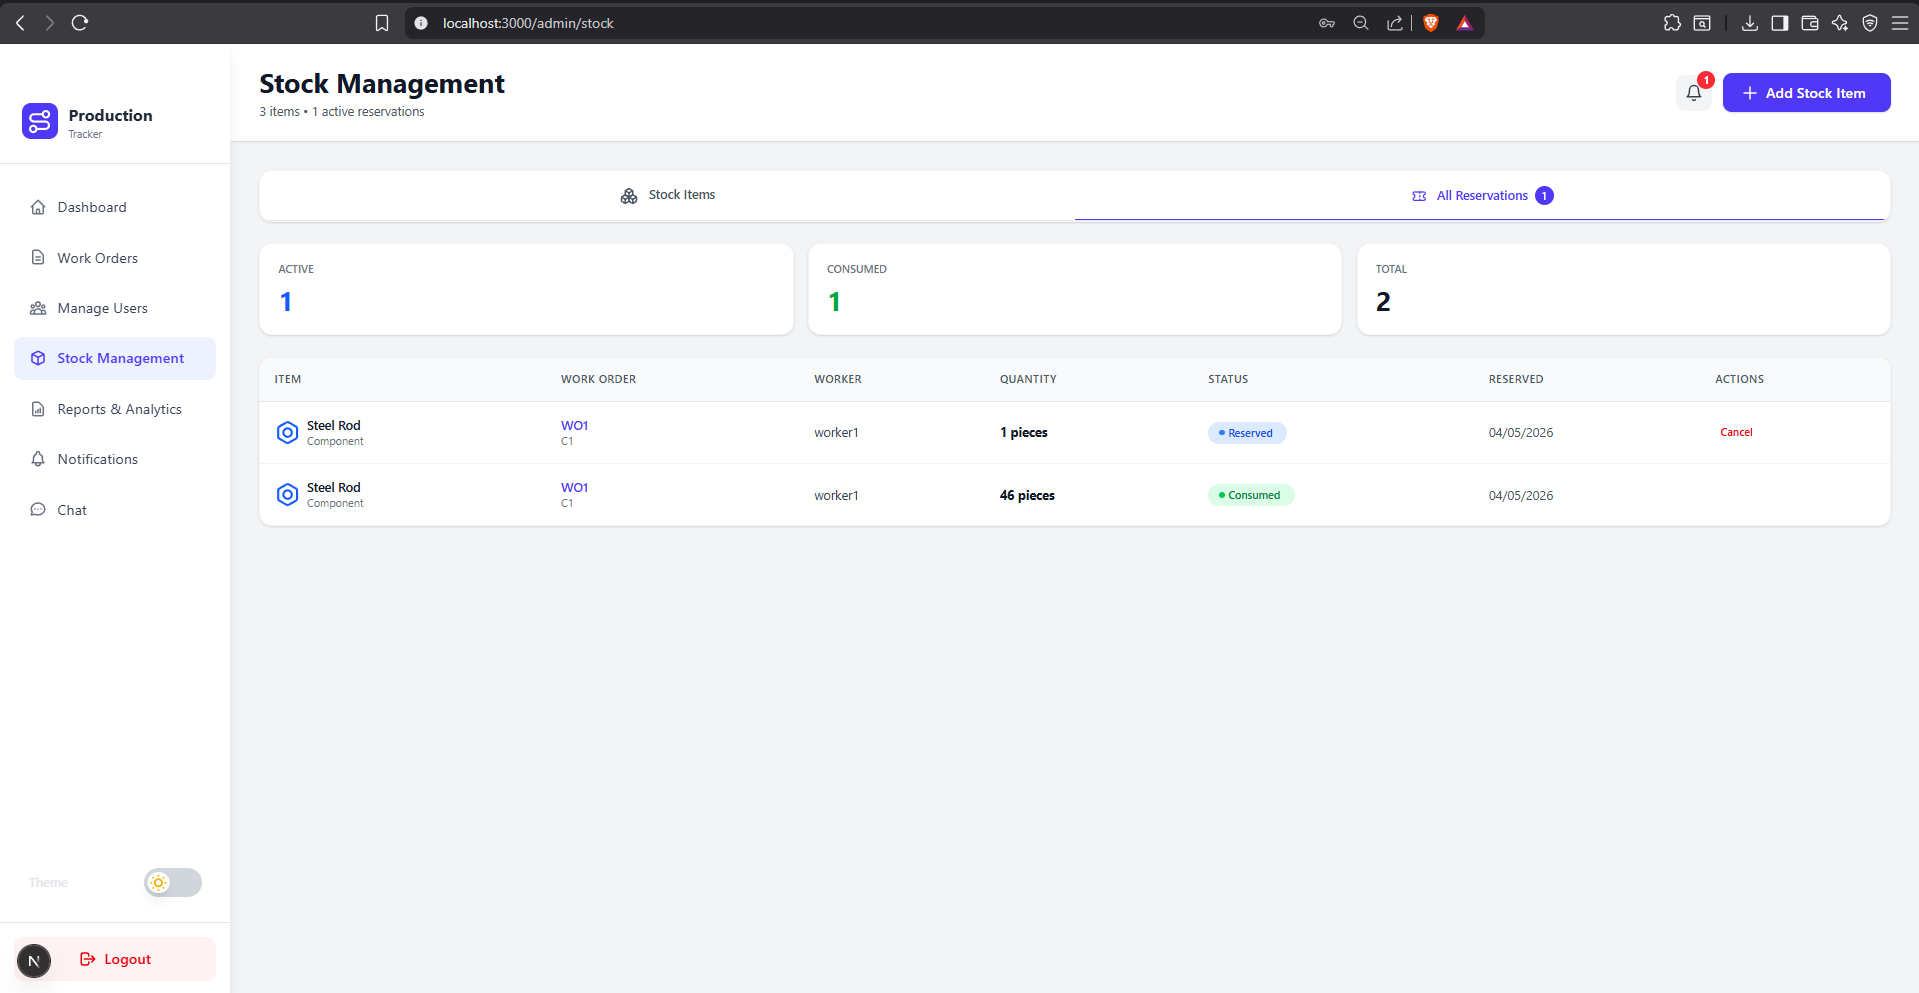
\includegraphics[width=\textwidth,keepaspectratio]{pictures/inventory reservations admin view.png}
        \caption{Inventory Reservations Admin View}
        \label{fig:inventory-reservations-admin-view}
    \end{minipage}

\end{figure}
 The figures \ref{fig:inventory-worker-view} and \ref{fig:inventory-reservations-worker-view} show the inventory interfaces for workers, enabling them to view available stock and manage their reservations effectively.
\begin{figure}[H]
    \centering

    \begin{minipage}[t]{0.48\textwidth}
        \centering
        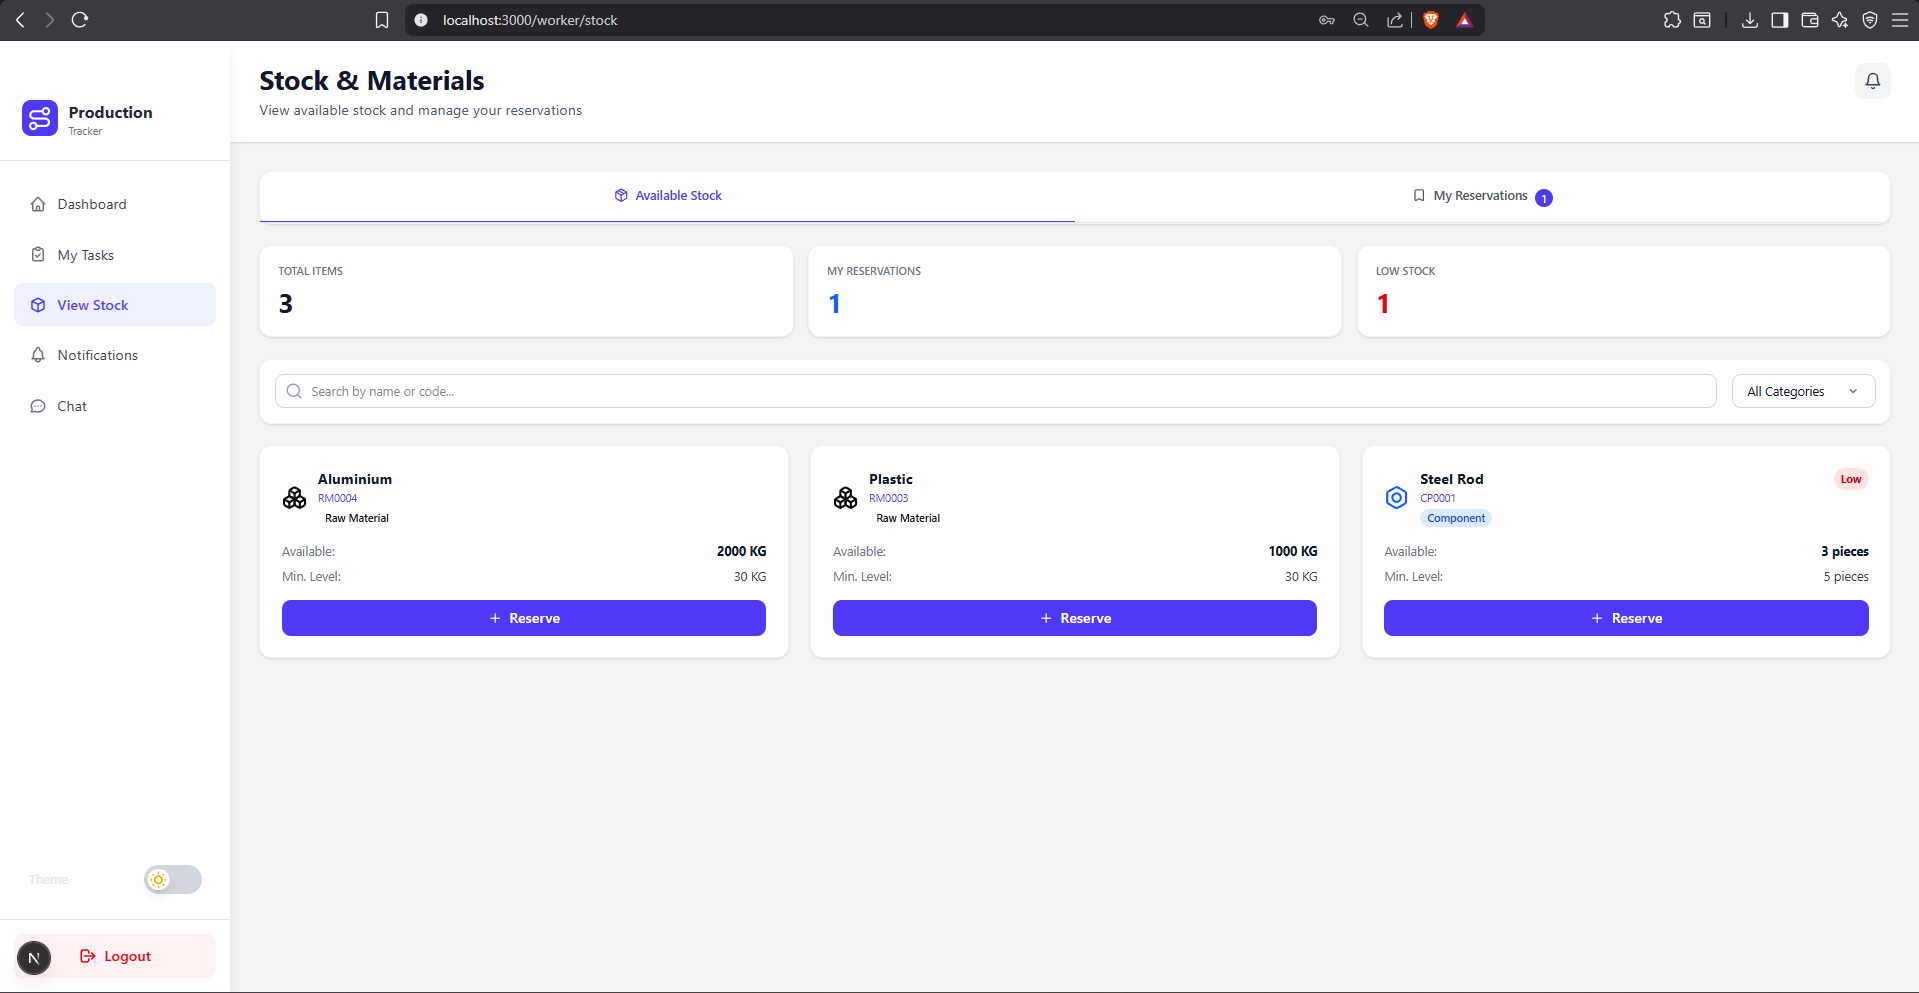
\includegraphics[width=\textwidth,keepaspectratio]{pictures/inventory worker view.png}
        \caption{Inventory Worker View}
        \label{fig:inventory-worker-view}
    \end{minipage}
    \hfill
    \begin{minipage}[t]{0.48\textwidth} 
        \centering
        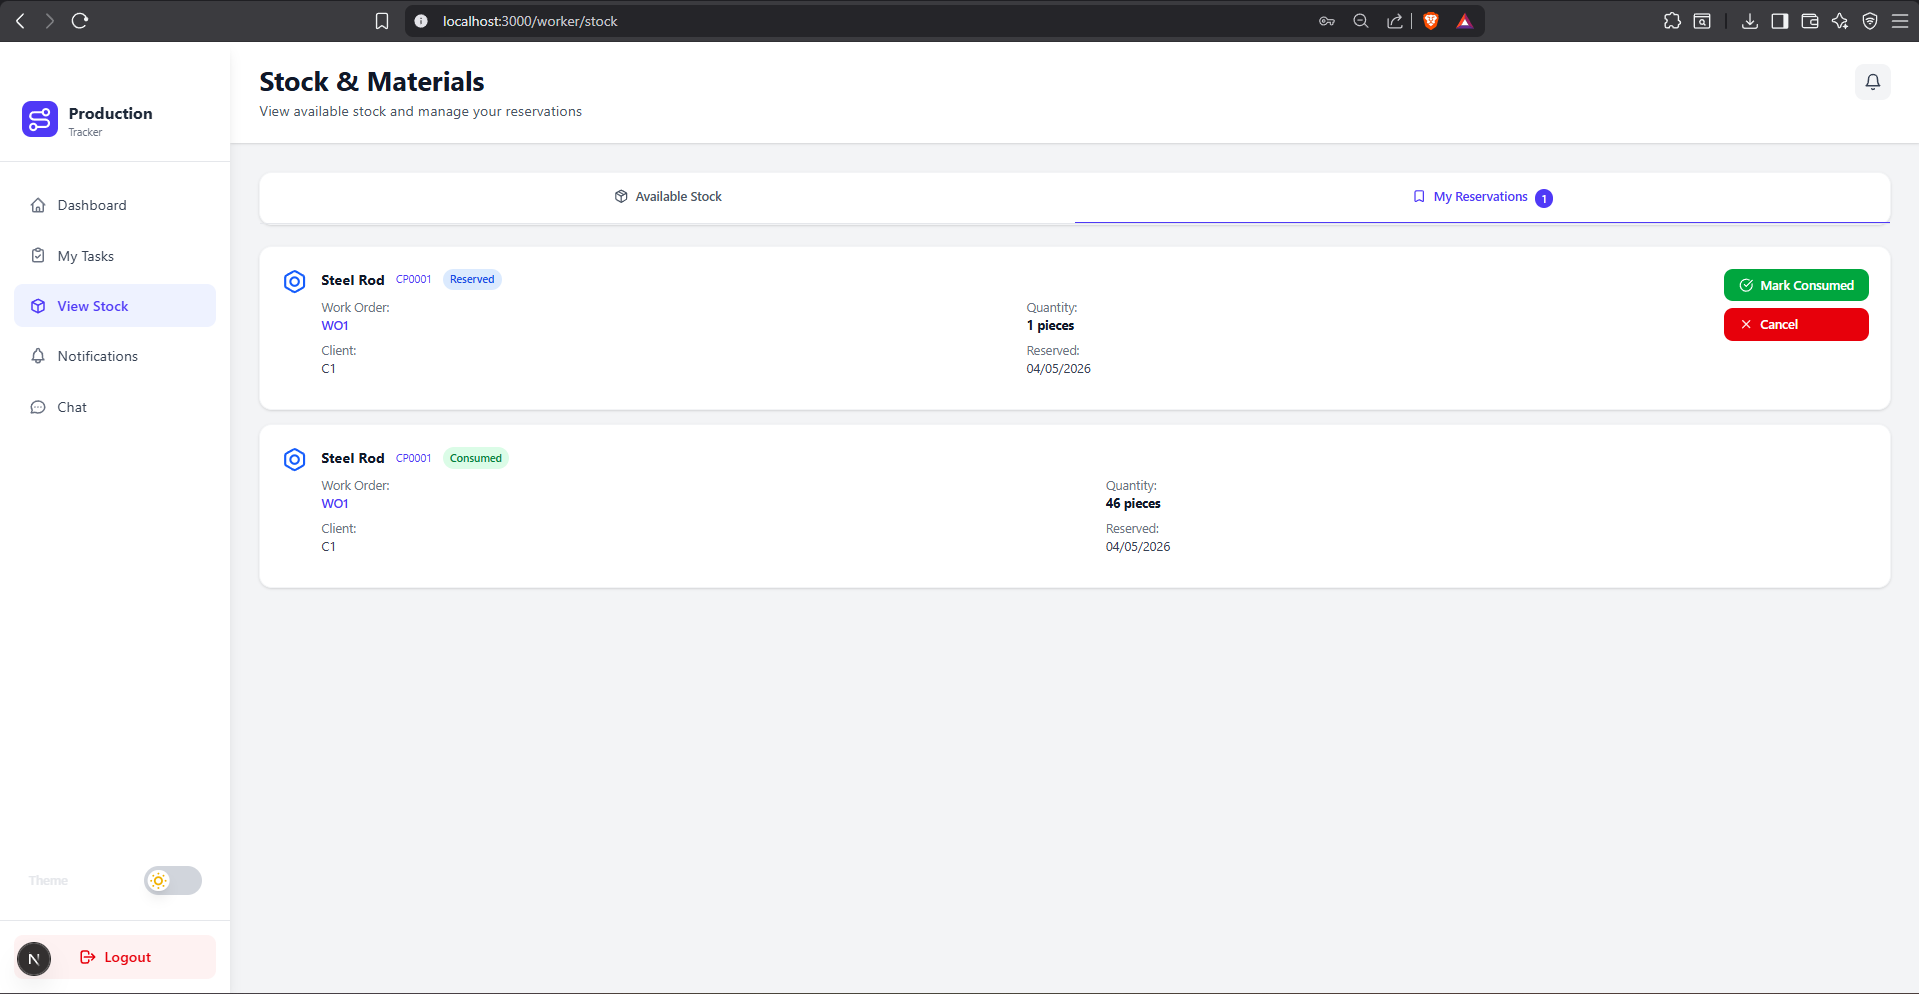
\includegraphics[width=\textwidth,keepaspectratio]{pictures/inventory reservations worker view.png}
        \caption{Inventory Reservations Worker View}
        \label{fig:inventory-reservations-worker-view}
    \end{minipage}

\end{figure}
\section{Conclusion}
\label{sec:release1-conclusion}

The first release completed the core features that formed the foundation of the Production Tracker software, by providing security through the implementation of authentication processes, building the core functionality that formed the production flow process, and finally, implementing inventory management. These three sprints lasted 21 days each, giving a total of 63 days, after which the second release will be covered in the next chapter.
